\documentclass[a4paper,man,natbib,12pt,apacite]{apa6}\usepackage[]{graphicx}\usepackage[]{color}
%% maxwidth is the original width if it is less than linewidth
%% otherwise use linewidth (to make sure the graphics do not exceed the margin)
\makeatletter
\def\maxwidth{ %
  \ifdim\Gin@nat@width>\linewidth
    \linewidth
  \else
    \Gin@nat@width
  \fi
}
\makeatother

\definecolor{fgcolor}{rgb}{0.345, 0.345, 0.345}
\newcommand{\hlnum}[1]{\textcolor[rgb]{0.686,0.059,0.569}{#1}}%
\newcommand{\hlstr}[1]{\textcolor[rgb]{0.192,0.494,0.8}{#1}}%
\newcommand{\hlcom}[1]{\textcolor[rgb]{0.678,0.584,0.686}{\textit{#1}}}%
\newcommand{\hlopt}[1]{\textcolor[rgb]{0,0,0}{#1}}%
\newcommand{\hlstd}[1]{\textcolor[rgb]{0.345,0.345,0.345}{#1}}%
\newcommand{\hlkwa}[1]{\textcolor[rgb]{0.161,0.373,0.58}{\textbf{#1}}}%
\newcommand{\hlkwb}[1]{\textcolor[rgb]{0.69,0.353,0.396}{#1}}%
\newcommand{\hlkwc}[1]{\textcolor[rgb]{0.333,0.667,0.333}{#1}}%
\newcommand{\hlkwd}[1]{\textcolor[rgb]{0.737,0.353,0.396}{\textbf{#1}}}%

\usepackage{framed}
\makeatletter
\newenvironment{kframe}{%
 \def\at@end@of@kframe{}%
 \ifinner\ifhmode%
  \def\at@end@of@kframe{\end{minipage}}%
  \begin{minipage}{\columnwidth}%
 \fi\fi%
 \def\FrameCommand##1{\hskip\@totalleftmargin \hskip-\fboxsep
 \colorbox{shadecolor}{##1}\hskip-\fboxsep
     % There is no \\@totalrightmargin, so:
     \hskip-\linewidth \hskip-\@totalleftmargin \hskip\columnwidth}%
 \MakeFramed {\advance\hsize-\width
   \@totalleftmargin\z@ \linewidth\hsize
   \@setminipage}}%
 {\par\unskip\endMakeFramed%
 \at@end@of@kframe}
\makeatother

\definecolor{shadecolor}{rgb}{.97, .97, .97}
\definecolor{messagecolor}{rgb}{0, 0, 0}
\definecolor{warningcolor}{rgb}{1, 0, 1}
\definecolor{errorcolor}{rgb}{1, 0, 0}
\newenvironment{knitrout}{}{} % an empty environment to be redefined in TeX

\usepackage{alltt}
\usepackage{changepage}
\usepackage[english]{babel}
\usepackage[utf8x]{inputenc}
\usepackage{amsmath}
\usepackage{graphicx}
\usepackage{hyperref}
\usepackage{longtable}
\usepackage{varioref}
\usepackage[longnamesfirst]{natbib}
%\usepackage[natbibapa]{apacite}
\usepackage[colorinlistoftodos]{todonotes}
\usepackage{lineno}
\usepackage{listings}
\usepackage{longtable}
\usepackage{verbatim}
\usepackage[yyyymmdd,hhmmss]{datetime}

\newlength{\wideitemsep}
\setlength{\wideitemsep}{\itemsep}
\addtolength{\wideitemsep}{-10pt}
\let\olditem\item
\renewcommand{\item}{\setlength{\itemsep}{\wideitemsep}\olditem}


% New definition of square root:
% it renames \sqrt as \oldsqrt
\let\oldsqrt\sqrt
% it defines the new \sqrt in terms of the old one
\def\sqrt{\mathpalette\DHLhksqrt}
\def\DHLhksqrt#1#2{%
\setbox0=\hbox{$#1\oldsqrt{#2\,}$}\dimen0=\ht0
\advance\dimen0-0.2\ht0
\setbox2=\hbox{\vrule height\ht0 depth -\dimen0}%
{\box0\lower0.4pt\box2}}
\makeatletter
\newread\pin@file
\newcounter{pinlineno}
\newcommand\pin@accu{}
\newcommand\pin@ext{pintmp}
% inputs #3, selecting only lines #1 to #2 (inclusive)
\newcommand*\partialinput [3] {%
  \IfFileExists{#3}{%
    \openin\pin@file #3
    % skip lines 1 to #1 (exclusive)
    \setcounter{pinlineno}{1}
    \@whilenum\value{pinlineno}<#1 \do{%
      \read\pin@file to\pin@line
      \stepcounter{pinlineno}%
    }
    % prepare reading lines #1 to #2 inclusive
    \addtocounter{pinlineno}{-1}
    \let\pin@accu\empty
    \begingroup
    \endlinechar\newlinechar
    \@whilenum\value{pinlineno}<#2 \do{%
      % use safe catcodes provided by e-TeX's \readline
      \readline\pin@file to\pin@line
      \edef\pin@accu{\pin@accu\pin@line}%
      \stepcounter{pinlineno}%
    }
    \closein\pin@file
    \expandafter\endgroup
    \scantokens\expandafter{\pin@accu}%
  }{%
    \errmessage{File `#3' doesn't exist!}%
  }%
}
\makeatother
\npdecimalsign{.}
\newcommand{\cil}[1]{\todo[inline, color=green!40]{#1}}
\newcommand{\cm}[1]{\todo[color=green!40]{#1}}
\newcommand{\cmb}[1]{\todo[color=blue!40]{\lstinline|#1|}}
\title{Intelligence and Age at First Intercourse: Cause or Confound?}
\shorttitle{Intelligence and AFI}
\author{S. Mason Garrison and Joseph Lee Rodgers}
\affiliation{Vanderbilt University}
\addtolength{\marginparwidth}{6cm}
\addtolength{\paperwidth}{\marginparwidth-1cm}
%\addtolength{\marginparsep}{2mm}
\abstract{Your abstract here.\\\today\ at \currenttime}
\authornote{This material is based upon work that has been supported by the National Science Foundation Graduate Research Fellowship Program under Grant No. (DGE-1445197) and various means of institutional support from the following universities: University of British Columbia \& Vanderbilt University.}
\IfFileExists{upquote.sty}{\usepackage{upquote}}{}
\begin{document}
\maketitle
%\linenumbers%\section{Introduction}\section{ }\vspace{-.8cm}
\cmb{content/introduction.txt}Anecdotal evidence from the popular media, such as MTV's reality television franchise, \textit{16 and Pregnant}\nocite{mtv}, suggests that teenage sexual involvement is on the rise. Academic research supports such evidence; age at first intercourse (AFI) is indeed declining and has for some time \citep{bozon2003,finer2007trends,Kann2014}. Early AFI is associated with downstream consequences, including lower educational attainment \citep{Harden2012,Spriggs2008,Wellings2001}, failure to meet education and career goals \citep{halpern2000smart}, increased risk of teenage pregnancy \citep{Leitenberg2000,Wellings2001}, and increased rates of sexually transmitted infections \citep[STIs;][]{kaestle2005young}. Moreover, beyond the obvious benefit of avoiding those negative outcomes, delaying AFI is associated with greater relationship satisfaction, perception of increased attractiveness, and higher household income \citep{Harden2012}. Because many of the negative consequences above are severe and long-reaching, it is important to identify the causal mechanisms associated with early AFI. One potential factor exerting causal influence on AFI is intelligence.

Higher levels of intelligence are associated with delaying first intercourse \citep{halpern2000smart,mott1983early,Paul2000,Woodward2001}, and also with delay of less-intimate sexual involvement \citep{halpern2000smart}. Specifically, intelligent individuals may delay intercourse to ``safeguard'' their futures \citep{kirby2002effective, manlove1998influence, raffaelli2003sexual}. They perceive the risks associated with early intercourse, (\eg, pregnancy, STIs) to have life- and career-shattering outcomes \citep{halpern2000smart,harden2011don}. Although the link between intelligence and AFI has face validity, and has been confidently asserted (or often implied) as a causal link, a fundamental confound exists in most past research that limits our ability to infer causality.

Virtually all of the AFI-intelligence literature has used between-family designs. In analysis of data from such designs, a number of genetic and environmental influences, such as education and maternal intelligence are confounded \citep{DOnofrio2013,harden2014genetic,Lahey2010,Rodgers2000}. By ignoring such confounds, the source of variance is ambiguous, and researchers that attribute the source to specific between- or within-family sources risk misattributions of causality \citep{Rowe1997,Rutter2007}. There is the potential for this type of confound in virtually all past research on the link between intelligence and AFI \citep{harden2011don,harden2014genetic,plomin2004intelligence,rodgers1999nature,rodgers1994df}. Thus, we need to critically evaluate whether intelligence has a causal influence on AFI or is rather a theoretically attractive confound. To resolve some of these methodological challenges, we use design innovations that emerge from the excellent cross-generational and longitudinal structure of the National Longitudinal Survey of Youth (NLSY; we use both the original NLSY79 survey and the NLSY-Children survey, described below).
%
\section{Cause or Confound?}
There are numerous theories that address the motivations for adolescents' initiation of first intercourse (see \citealp{Rodgers1996} or \citealp{Buhi2007} for reviews), and even more specific precursors to first intercourse \citep{Buhi2007,DOnofrio2010,kirby2002antecedents,miller1997timing,santelli1992risk}. Many of these theories emphasize biology/genetics, as adolescent pubertal development (and associated hormone changes) drives the onset of sexual behavior \citep{miller1999dopamine,udry1979age,udry1994nature}. Other theoretical frameworks use social/environmental processes to explain developing sexual involvement in adolescence, such as Social Learning \citep{diblasio1990adolescent,hogben1998using}, where social norms affect the likelihood of early sexual behavior; or Social Control theory \citep{hirschi2002causes}, where societal and cultural influences reduce the likelihood that individuals will act on their natural tendency toward sexual involvement. Under these environmental theories the underlying biology is typically ignored (\eg, Social Control theory), whereas under many of the biological/genetic theories, the environmental components are often ignored.

However, numerous articles have also advocated integrative models \citep[See][]{harden2008rethinking,harden2014genetic,udry1995sociology}. The integrative Biopsychosocial Model acknowledges both genetic and environmental contributions to human behavior \citep{Engel1977,petersen1987nature,rodgers1999nature}. Indeed, biology, psychology, and society/culture jointly influence adolescents' decisions to engage in sexual intercourse \citep{Meschke2000,zimmer2008ten}.
%
\subsection{Intelligence as Cause}
The short-term risks of early AFI are primarily negative, whereas the rewards for delay are primarily positive. These consequences extend into adulthood -- early AFI has been related to adult delinquency \citep{harden2008rethinking}, anti-social behavior, and substance abuse \citep{boislard2011individual}, whereas those with delayed AFI have higher household incomes in adulthood \citep{Harden2012}. It is intuitively appealing to believe that intelligent individuals are more likely to observe this potential risk-reward trade off, and through volition act upon such observations by delaying first intercourse. Accordingly, intelligent individuals perceive the consequences of early AFI to negatively influence their careers \citep{halpern2000smart,harden2011don}.

Indeed, most of the literature has contributed to the expectation that intelligence is causally connected to AFI. Those with higher educational goals delay their first intercourse \citep{boislard2011individual,schvaneveldt2001academic}, whereas those who engaged in early sexual intercourse reduced their educational goals compared to earlier higher goals \citep{schvaneveldt2001academic}. Beyond academic goals, those with a greater affinity for risk and those who perceive benefits from teen-pregnancy are more likely to engage in risky sexual activities \citep{raffaelli2003sexual}. A greater understanding of the risks associated with sexual intercourse, such as HIV transmission, is also associated with delayed AFI \citep{mathews2009predictors}.

Smarter adolescents are more likely to report delayed intercourse \citep{halpern2000smart,mott1983early,Paul2000,Woodward2001}. Besides delaying first intercourse, smarter individuals appear to postpone all sexual/romantic activity \citep{halpern2000smart}. Such blanket delays may be a proactive attempt to avoid ``gateway'' activities that might lead to intercourse. Thus, many researchers have concluded that ``[h]igher intelligence operates as a protective factor against early sexual activity during adolescence, and lower intelligence, to a point, is a risk factor.'' \citep[][p. 213]{halpern2000smart}.

However, \citet{halpern2000smart} and many of the other studies we have referenced \citep[e.g.,][]{mathews2009predictors,miller1997timing,Paul2000} used between-family, typically cross-sectional, designs. Such designs cannot logically distinguish between processes that act to create differences between families and processes that create differences among family members \citep{Lahey2010,Rodgers2000}. Thus the previous studies do no provide conclusive evidence that intelligence is the causal influence behind the AFI-intelligence relationship. Logically, other alternatives are that AFI has a causal link to intelligence (which is unlikely, for the obvious theoretical reasons, including that a child's intelligence precedes AFI in time) or that other confounds cause these two outcomes to correlate, but not causally. There are dozens, perhaps hundreds, of such confounds that can logically contend to explain the link between child intelligence and AFI; we review those confounds in the next section.
%
\subsection{Intelligence as a Confound}
An equally valid set of explanations exist in which intelligence is not the causal factor behind the AFI-intelligence relationship, but rather one of dozens of correlated potentially explanatory processes. Instead, various confounds including family level selection effects, or third variables at the individual or family level could be causing the relationship. Indeed many such findings that link intelligence with various outcomes are quite possibly the result of misattributing between-family confounds to individual-level and within-family causes.

The relationship between birth order and intelligence is a classic example of this misattribution \citep[See][]{damian2015associations,Rodgers2000,rodgers2014birth}. We briefly review that research arena here, because it illustrates the same challenge that occurs in studying the link between intelligence and AFI. 

Between-family studies that rely on cross-sectional data have consistently found that first born children have higher IQs than later born children \citep{belmont1973birth,zajonc1976family}. Yet within-family studies have typically found a non-significant relationship (\citealp{berbaum1980intellectual,galbraith1982sibling,retherford1991birth,Rodgers2000}; also see \citealp{barclay2015within} and \citealp{bjerkedal2007intelligence} for recent exceptions that have found small, but significant within-family effects in large national studies). Moreover, when designs that can distinguish within- and between-family variance have been conducted, the methodological source of the IQ-birth order effects have emerged from the between-family variance \citep{black2011older,rodgers1984confluence,Rodgers2000,Wichman2006,Wichman2007}. Potential causes of this confound include maternal age at first birth, parental IQ, parental education, and SES \citep[][also see \citep{Anastasi1956} for an insightful overview, written prior to the IQ-birth order debate.]{page1979family,Rodgers2001admixture,Rodgers2008AJS}.

In summary, if there is a valid within-family link between intelligence and birth order (which is, definitionally, a within-family variable), it is at one extreme of small magnitude and only detectable in large national datasets, and at the other extreme non-existent (even in large U.S. datasets). Similarly, the link between intelligence and AFI may be mostly or completely spurious. For example, one study found that socioeconomic status is associated with the onset of first intercourse \citep{Lammers2000}, which implicates a between-family process as explanatory of much of the negative consequence early AFI and teenage pregnancy.

\cil{Is the content below cut?\\
\citep{geronimus1992socioeconomic}, and is correlated with intelligence \citep{murray1998income,Neisser1996,Strenze2007}. Parental intelligence and parental education are also linked with child intelligence \citep{Bouchard2004,devlin1997heritability,mercy1982familial}, and pose viable alternative explanations in which parents could be influencing, or even actively dissuading, their children from engaging in early intercourse. For example, daughters whose mothers communicated frequently about the risk associated with sexual intercourse were less likely to have unprotected sex and engaged in sex less frequently \citep{hutchinson2003role}. Thus it could be that intelligent mothers, not intelligent children, are the ones recognizing the consequences of early intercourse and acting accordingly. In order to better understand the causal relation between intelligence and AFI, we need to be able to untangle between- and within-family processes, using both data and designs that have the ability to separate these sources of variance.}
\subsection{Prior Within-Family Analyses} Two past studies have explicitly separated between- and within-family influences on the AFI-intelligence relationship \citep{harden2011don,nedelec2012exploring}. Harden and Mendle used 536 same-sex twin pairs from the Add Health Study to ``test[ ] whether relations between intelligence, academic achievement and age at first sex were due to unmeasured genetic and environmental differences between families.'' Twins who differed in their intelligence or their academic achievement did not differ in their age at first intercourse. They concluded that ''the association between intelligence and age at first sex could be attributed entirely to \textit{unmeasured environmental differences between families}.''(italics added, our own emphasis). Nedelec, Schwartz, Connolly, and Beaver (\citeyear{nedelec2012exploring}) conducted an exploratory analysis of MZ twin pairs from the same sample used by Harden and Mendle, using intelligence difference scores to predict various social outcomes. They found consistent null results, though their samples were small and their statistical analyses were substantially underpowered.


\section{Present Study}
\begin{itemize}
\item We wanted to know whether the Harden \& Mendle (2011) results would hold using a different design and data set.\smallskip
\item We examined the relationship between AFI and Intelligence using siblings and their children from a multigenerational nationally representative sample.\smallskip
\item Specifically, we addressed the following questions:\smallskip
\begin{itemize}\item Does intelligence (mother or child) predict child AFI, after controlling for gene and environmental confounds?\smallskip
\item Is this relationship consistent between-- and within--families?
\end{itemize}\end{itemize}

\section{Methods}\cmb{content/methods.txt}\input{content/methods.txt}


\cmb{content/Gen1measure.txt}\input{content/Gen1measure.txt}

\cmb{content/Gen2measure.txt}\input{content/Gen2measure.txt}

\section{Results}\cmb{content/results.txt}We examined the relationship between AFI and intelligence using two designs: a between-family design, and a combination between- and within-family design (which includes between-family variance in the differences between the family means, and within-family variance in the sibling/cousin differences). The results are organized by those two designs. The between-family analyses report the relationships between the within-family average AFI and various measures of ability. The combination between-family/within-family analyses add to the between-family analyses the difference scores, testing whether differences in AFI can be explained by differences in various measures of ability, controlling for the between-family variance.
%\subsection{Between vs. Within Illustration}
%\cmb{content/results_meancomp.txt}\input{content/results_meancomp.txt}

\subsection{Between Family Anlayses}\cmb{content/results_between.txt}First, we examined the between-family results. We tested whether the family average of Gen2 AFI could be predicted by the family averages of Gen1 intelligence and of Gen2 intelligence. We evaluated the influences both independently and simultaneously. All intelligence scores have been standardized by generation ($\overline{g} = 0$, sd $= 1$), prior to averaging by household. AFI scores have been standardized by gender ($\overline{\mathrm{AFI}} = 0$, sd $= 1$), prior to averaging by household. In Tables \ref{table_Mean_Mom_Intelligence_Mean_Child_AFI_9} - \ref{table_Mean_Joint_Intelligence_Mean_Child_AFI_9}, we have reported results for three different linking methods:
\begin{itemize} 
\item The mixed model, which contains the firstborn child of each sister;
\item The daughters model, which contains the firstborn daughters; and 
\item The sons model, which contains the firstborn sons).\end{itemize}
In the spirit of transparency, we have reported all three methods. However, because all three linking methods reported similar findings, we will focus the results section on the mixed model and only discuss the other two methods when they deviate. We have also provided zero-order and pairwise semi-partial correlations for all between-family variables (Tables \ref{table_cor} and \ref{table_spcor_btw}), using the mixed-model data and the ppcor \R library \citep{kim2015ppcor}.

\subsubsection{Gen1 Mean Intelligence $\rightarrow$ Gen2 Mean AFI} Gen1 sister averages (NLSY79 mothers) of standardized AFQT scores were used to predict Gen2 averages of gender-standardized AFI. Table \ref{table_Mean_Mom_Intelligence_Mean_Child_AFI_9} displays the results by Gen2 category. The mixed model reports the averages of the firstborn child (both males and females) of each maternal sister (n $= 342$). A one-unit increase in the average standardized intelligence of the children's mothers predicted a statistically significant increase of $.013$ standard deviations in average Gen2 AFI. When we transform the coefficient into a standardized beta weight ($\beta_{Gen1 Intell} = .299$), a standard-deviation increase in the averaged mother's intelligence predicts a .299 standard-deviation increase in the average of the cousins' AFI. The adjusted R$^{2}$ was .087.

\subsubsection{Gen2 Mean Intelligence $\rightarrow$ Gen2 Mean AFI} Gen2 averages of standardized intelligence scores were used to predict Gen2 averages of gender\hyph standardized AFI. Table \ref{table_Mean_Child_Intelligence_Mean_Child_AFI_9} displays the results by Gen2 category. The mixed model reports the averages of the firstborns of each of the NLSY79 mothers (sisters) (n $= 344$). A one-unit increase in the average standardized intelligence of the children predicted a statistically significant $\approx .075$ standard-deviation increase in average Gen2 cousins' AFI. When we transform the coefficient into a standardized beta weight ($\beta_{Gen2 Intell} = .128$), a standard-deviation increase in the averaged cousins' intelligence predicts a .128 standard-deviation increase in the average of the cousins' AFI. The adjusted R$^{2}$ was $.014$.

\subsubsection{Joint Mean Intelligence $\rightarrow$ Gen2 Mean AFI} Results from the Gen1 maternal sister averages of standardized AFQT scores and Gen2 averages of standardized intelligence scores predicting Gen2 averages of gender\hyph standardized AFI are displayed in Table \ref{table_Mean_Joint_Intelligence_Mean_Child_AFI_9}. In the mixed model, Gen1 (maternal) intelligence was significantly associated with Gen2 AFI (p $< .01$), while Gen2 (child) intelligence was not significantly associated with Gen2 AFI. A one-unit increase in the average standardized intelligence of the children's mothers predicted $.013$ standard-deviation increase in average Gen2 AFI, after controlling for Gen2 cousin averages of standardized intelligence scores. When we transform the coefficients into standardized beta weights ($\beta_{Gen1 Intell} = .303$; $\beta_{Gen2 Intell} = -.003$), a standard-deviation increase in the averaged mother's intelligence predicts a .303 standard-deviation increase in the average of the cousins' AFI. The adjusted R$^{2}$ was $.086$. The total variance explained by the Joint model ($R^{2}$ = 9.1$\%$) is nearly identical to the Gen1 model($R^{2}$=9$\%$). Gen2 intelligence explains an additional .1\% of the variance.

When we broaden our sample to all Mother-Child pairs, we see that the relationship between Gen 2 intelligence and Gen2 AFI is small $(r =.139)$, and smaller than the relationship between Gen1 intelligence and Gen2 AFI $(r=.215$; see Figure \ref{plot_gen2_afi}).

\begin{landscape}
\begin{longtable}{@{\extracolsep{5pt}}lccc} 
\caption{Between-Family: Gen1 Intelligence Predicts Gen2 AFI}\label{table_Mean_Mom_Intelligence_Mean_Child_AFI_9}
\\[-1.8ex]\hline 
\hline \\[-3.8ex] 
& \multicolumn{3}{c}{\textit{Dependent variable:} Average of Gen2 AFI} \\ 
\cline{2-4}
\partialinput{10}{21}{../Common/content/tables/table_Mean_Mom_Intelligence_Mean_Child_AFI_9.tex}\\[-7ex]
\textit{Notes:}  & \multicolumn{3}{r}{$^{*}$p$<$0.1; $^{**}$p$<$0.05; $^{***}$p$<$0.01} \\[2ex]
& \multicolumn{3}{r}{\parbox{.6\linewidth}{\footnotesize Gen1-sister averages (NLSY79 mothers) of standardized AFQT scores predict Gen2 averages of gender-standardized AFI.}} \\ 
\end{longtable}\pagebreak

\begin{longtable}{@{\extracolsep{5pt}}lccc} 
\caption{Between-Family: Gen2 Intelligence Predicts Gen2 AFI}\label{table_Mean_Child_Intelligence_Mean_Child_AFI_9}
\\[-1.8ex]\hline 
\hline \\[-3.8ex] 
& \multicolumn{3}{c}{\textit{Dependent variable:} Average of Gen2 AFI} \\ 
\cline{2-4}
\partialinput{10}{21}{../Common/content/tables/table_Mean_Child_Intelligence_Mean_Child_AFI_9.tex}\\[-7ex]
\textit{Notes:}  & \multicolumn{3}{r}{$^{*}$p$<$0.1; $^{**}$p$<$0.05; $^{***}$p$<$0.01} \\[2ex]
& \multicolumn{3}{r}{\parbox{.6\linewidth}{\footnotesize Gen2-cousin averages of standardized intelligence scores predict Gen2 averages of gender-standardized AFI.}} \\ 
\end{longtable}\pagebreak

\begin{longtable}{@{\extracolsep{5pt}}lccc} 
\caption{Between-Family: Gen1 \& Gen2 Intelligence Predict Gen2 AFI}\label{table_Mean_Joint_Intelligence_Mean_Child_AFI_9}
\\[-1.8ex]\hline 
\hline \\[-3.8ex] 
& \multicolumn{3}{c}{\textit{Dependent variable:} Average of Gen2 AFI} \\ 
\cline{2-4}
\partialinput{10}{22}{../Common/content/tables/table_Mean_Joint_Intelligence_Mean_Child_AFI_9.tex}\\[-7ex]
\textit{Notes:}  & \multicolumn{3}{r}{$^{*}$p$<$0.1; $^{**}$p$<$0.05; $^{***}$p$<$0.01} \\[2ex]
& \multicolumn{3}{r}{\parbox{.6\linewidth}{\footnotesize Gen1-sister averages (NLSY79 mothers) of standardized AFQT scores and Gen2-cousin averages of standardized intelligence scores predict Gen2 averages of gender-standardized AFI.}} \\ 
\end{longtable}


\subsection{Within Family Analyses}
\cmb{content/results_between.txt}We replicated the between-family analyses reported in the previous subsection, using within-family difference scores and means. Using the discordant sibling model, we predicted the differences in Generation 2 AFI as a function of differences in intelligence, controlling for means of the outcomes and predictors. We ran three series of models, where we examined the individual and then joint influence of Gen1 intelligence and Gen2 intelligence. Moreover, within each series we included three Generation 2 linking method variants, just as we did in the between family analyses: Mixed model reports the differences of the first borns of each sister, the Daughters model reports the differences of the first born girls, and the Sons model reports the differences of the first born sons.

\subsubsection{Gen1 Intelligence Differences $\rightarrow$ Gen2 AFI Differences} 
Generation 1 sister differences in standardized AFQT scores were used to predict Generation 2 differences of gender standardized AFI, controlling for Generation 1 sister averages of standardized AFQT scores and Gen2 averages of gender standardized AFI. Table \ref{table_Dif_Mom_Intelligence_Dif_Child_AFI_9} displays the results by Generation 2 linking method. The Mixed model reports the averages and differences of the first borns of each sister (n $= 336$), the Daughters model reports the averages and differences of the first born girls (n $= 258$), and the Sons model reports the averages and differences of the first born sons (n $= 278$). All three models reveal similar results. Generation 2 averages of gender standardized AFI (between-family measures) were significant predictors of Gen2 differences in gender standardized AFI (p $< .01$), across all three linking methods. A one unit increase in the average gender standardized AFI predicted $\approx 0.34$ standard deviation increase in average Gen2 AFI difference, controlling for all over variables in the model. 

In the Sons model, the Generation 1 sister average of standardized AFQT scores was a significant predictor of differences in Gen2 AFI (p $< .01$). A one unit increase in the average standardized intelligence of the children's mothers predicted $\approx .0083$ decrease in the AFI difference between siblings. All other variables were not significant, including all kin difference variables (the within-family measures). Note that this result is somewhat anomalous, because it is in the opposite direction to the other results. The adjusted R$^{2}$ varied slightly by Generation 2 linking method (Mixed $= .066$, Daughters $= .072$, Sons $= .106$).

\subsubsection{Gen2 Intelligence Differences $\rightarrow$ Gen2 AFI Differences}
Gen2 cousin differences in standardized intellectual ability scores were used to predict Gen2 differences of gender standardized AFI, controlling for Gen2 cousin averages of standardized ability scores and gender standardized AFI (to account for between-family variance). Table \ref{table_Dif_Kid_Intelligence_Dif_Child_AFI_9} displays the results by Generation 2 categories. The Mixed model reports the averages and differences of the first borns of each sister (n $= 291$), the Daughters model reports the averages and differences of the first born girls (n $= 223$), and the Sons model reports the averages and differences of the first born sons (n $= 238$). All three models reveal similar results. Gen2 averages of gender standardized AFI were significant predictors of Generation 2 differences in gender standardized AFI (p $< .01$), across all three linking methods. A one unit increase in the average gender standardized AFI predicted $\approx 0.38$ standard deviation increase in average Gen2 AFI difference, controlling for all over variables in the model. 

In the Sons model, the Generation 2 cousin average of standardized ability scores was a significant predictor of differences in Generation 2 AFI (p $< .05$). A one unit increase in the average standardized intelligence of the children predicted $\approx .107$ decrease in the AFI difference between siblings (again, the Sons model result is in the opposite direction to other results). All other variables were not significant, including all kin difference variables. The adjusted R$^{2}$ varied slightly by Generation 2 linking method (Mixed $= .103$, Daughters $= .121$, Sons $= .132$).

\subsubsection{Joint Intelligence Differences $\rightarrow$ Gen2 AFI Differences}
Generation 1 sister differences in standardized AFQT scores and Gen2 cousin differences in standardized intellectual ability scores were used simultaneously to predict Generation 2 differences of gender standardized AFI, controlling for Generation 1 sister averages of standardized AFQT scores, Gen2 cousin averages of standardized ability scores, and Gen2 cousin averages of gender standardized AFI. Table \ref{table_Dif_Joint_Intelligence_Dif_Child_AFI_9} displays the results by Generation 2 categories. The Mixed model reports the averages and differences of the first borns of each sister (n $= 285$), the Daughters model reports the averages and differences of the first born girls (n $= 217$), and the Sons model reports the averages and differences of the first born sons (n $= 235$). All three models reveal similar results. Gen2 averages of gender standardized AFI were significant predictors of Generation 2 differences in gender standardized AFI (p $< .01$), across all three linking methods. A one unit increase in the average gender standardized AFI predicted $\approx 0.38$ standard deviation increase in Generation 2 AFI difference, controlling for all over variables in the model. 

All other variables were not significant, including all kin difference variables. The adjusted R$^{2}$ varied slightly by Generation 2 linking method (Mixed $= .090$, Daughters $= .105$, Sons $= .131$).\\
\begin{landscape}
\begin{longtable}{@{\extracolsep{5pt}}lccc} 
\caption{Gen1 Intelligence Differences $\rightarrow$ Gen2 AFI Differences}\label{table_Dif_Mom_Intelligence_Dif_Child_AFI_9}
\\[-1.8ex]\hline 
\hline \\[-1.8ex] 
& \multicolumn{3}{c}{\textit{Dependent variable:} Differences in Gen2 Mean AFI} \\ 
\cline{2-4}
\partialinput{10}{24}{../Common/content/tables/table_Dif_Mom_Intelligence_Dif_Child_AFI_9.tex}
\end{longtable}\pagebreak

\begin{longtable}{@{\extracolsep{5pt}}lccc} 
\caption{Gen2 Intelligence Differences $\rightarrow$ Gen2 AFI Differences}\label{table_Dif_Child_Intelligence_Dif_Child_AFI_9}
\\[-1.8ex]\hline 
\hline \\[-1.8ex] 
& \multicolumn{3}{c}{\textit{Dependent variable:} Differences in Gen2 Mean AFI} \\ 
\cline{2-4}
\partialinput{10}{24}{../Common/content/tables/table_Dif_Child_Intelligence_Dif_Child_AFI_9.tex}
\end{longtable}\pagebreak

\begin{longtable}{@{\extracolsep{5pt}}lccc} 
\caption{Dif Joint Intelligence $\rightarrow$ Gen2 Dif AFI}\label{table_Dif_Joint_Intelligence_Dif_Child_AFI_9}
\\[-1.8ex]\hline 
\hline \\[-1.8ex] 
& \multicolumn{3}{c}{\textit{Dependent variable:} Differences in Gen2 Mean AFI} \\ 
\cline{2-4}
\partialinput{10}{26}{../Common/content/tables/table_Dif_Joint_Intelligence_Dif_Child_AFI_9.tex}
\end{longtable}\end{landscape}


\section{Discussion}



\newpage\section{Tables}\label{appen_tables}

\subsection{Descriptive Statistics}
\begin{longtable}{@{\extracolsep{5pt}}lcccccc}
\caption{Gen1 Summary Statistics by Sibling Status.}\label{table_summary_stats_sibinsampleg1}
\partialinput{2}{10}{table_summary_stats_sibinsampleg1.tex}
\end{longtable}\linebreak

\begin{longtable}{@{\extracolsep{5pt}}lcccccc}
\caption{Gen2 Summary Statistics by Sibling Status.}\label{table_summary_stats_sibinsampleg2}
\partialinput{2}{10}{table_summary_stats_sibinsampleg2.tex}
\end{longtable}\pagebreak
\npnoround
\begin{longtable}{@{\extracolsep{5pt}}lllcc}
\caption{Gen2 AFI by Gender, Race, and GenderxRace.}\label{table_afi_race_gender}
\partialinput{2}{18}{table_summary_stats_AFIRACEGENDER.tex}
\end{longtable}\pagebreak


\begin{longtable}{@{\extracolsep{5pt}}cc} 
\caption{Gen2 Measurement Model.}\label{table_gen2measurement_9}
\\[-1.8ex]\hline 
\hline \\[-1.8ex] 
 & g at Age 9.5 \\ 
\hline \\[-1.8ex] 
\partialinput{12}{34}{table_g2_9measurement.tex}
\end{longtable}\pagebreak

\begin{longtable}{@{\extracolsep{5pt}}cccccc} 
\caption{Gen2 Factor Loadings.}\label{table_g2loading_9}
\\[-1.8ex]\hline 
\hline \\[-1.8ex] 
 & Test & Estimate & S.E. & Est./.S.E. & P.Value \\  
\hline \\[-1.8ex] 
\partialinput{12}{17}{table_g2loading_9.tex}
\end{longtable}\pagebreak

\subsection{Between Family Analyses}
\begin{longtable}{@{\extracolsep{5pt}}lccc} 
\caption{Mean Gen1 Intelligence $\rightarrow$ Mean Gen2 AFI}\label{table_Mean_Mom_Intelligence_Mean_Child_AFI_9}
\partialinput{5}{24}{table_Mean_Mom_Intelligence_Mean_Child_AFI_9.tex}
\end{longtable}\pagebreak

\begin{longtable}{@{\extracolsep{5pt}}lccc} 
\caption{Mean Gen2 Intelligence $\rightarrow$ Mean Gen2 AFI}\label{table_Mean_Child_Intelligence_Mean_Child_AFI_9}
\partialinput{5}{24}{table_Mean_Child_Intelligence_Mean_Child_AFI_9.tex}
\end{longtable}\pagebreak

\begin{longtable}{@{\extracolsep{5pt}}lccc} 
\caption{Mean Joint Intelligence $\rightarrow$ Mean Gen2 AFI}\label{table_Mean_Joint_Intelligence_Mean_Child_AFI_9}
\partialinput{5}{26}{table_Mean_Joint_Intelligence_Mean_Child_AFI_9.tex}
\end{longtable}\pagebreak
\subsection{Within Family Analyses}
\begin{longtable}{@{\extracolsep{5pt}}lccc} 
\caption{Dif Gen1 Intelligence $\rightarrow$ Dif Gen2 AFI}\label{table_Dif_Mom_Intelligence_Dif_Child_AFI_9}
\partialinput{5}{28}{table_Dif_Mom_Intelligence_Dif_Child_AFI_9.tex}
\end{longtable}\pagebreak

\begin{longtable}{@{\extracolsep{5pt}}lccc} 
\caption{Dif Gen2 Intelligence $\rightarrow$ Dif Gen2 AFI}\label{table_Dif_Child_Intelligence_Dif_Child_AFI_9}
\partialinput{5}{28}{table_Dif_Child_Intelligence_Dif_Child_AFI_9.tex}
\end{longtable}\pagebreak

\begin{longtable}{@{\extracolsep{5pt}}lccc} 
\caption{Dif Joint Intelligence $\rightarrow$ Dif Gen2 AFI}\label{table_Dif_Joint_Intelligence_Dif_Child_AFI_9}
\partialinput{5}{32}{table_Dif_Joint_Intelligence_Dif_Child_AFI_9.tex}
\end{longtable}

\begin{comment}\section{Figures}\label{figures}

\begin{figure}
  \centering
    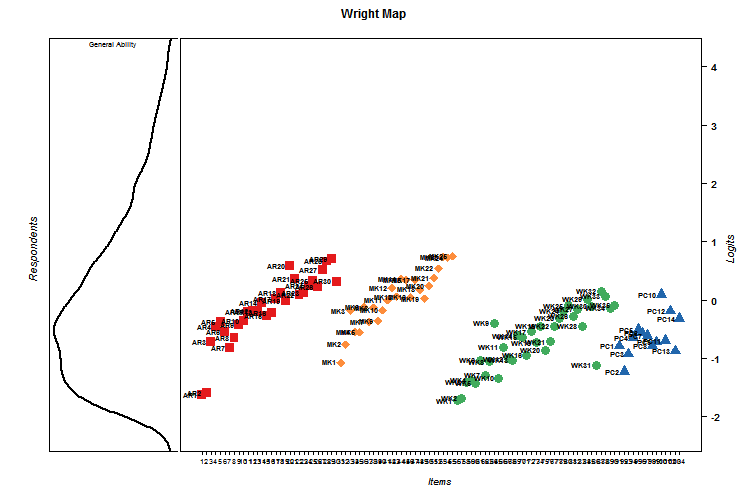
\includegraphics[height=.85\textwidth,angle=270]{G1wrightMap}
     \caption{Wright Map of Gen1 Cognitive Ability}\label{G1wrightMap}
\end{figure}\end{comment}
\appendix\label{appen}
\section{Age 10.5 Replication}\label{appen10}
\begin{longtable}{@{\extracolsep{5pt}}cc} 
\caption{Gen2 Measurement Model.}\label{table_gen2measurement_10}
\\[-1.8ex]\hline 
\hline \\[-1.8ex] 
 & g at Age 10.5 \\ 
\hline \\[-1.8ex] 
\partialinput{12}{34}{table_g2_10measurement.tex}
\end{longtable}\pagebreak

\begin{longtable}{@{\extracolsep{5pt}}cccccc} 
\caption{Gen2 Factor Loadings.}\label{table_g2loading_10}
\\[-1.8ex]\hline 
\hline \\[-1.8ex] 
 & Test & Estimate & S.E. & Est./.S.E. & P Value \\  
\hline \\[-1.8ex] 
\partialinput{12}{17}{table_g2loading_10.tex}
\end{longtable}\pagebreak
\subsection{Between Family Analyses}
\begin{longtable}{@{\extracolsep{5pt}}lccc} 
\caption{Mean Gen1 Intelligence $\rightarrow$ Mean Gen2 AFI}\label{table_Mean_Mom_Intelligence_Mean_Child_AFI_10}
\partialinput{5}{24}{table_Mean_Mom_Intelligence_Mean_Child_AFI_10.tex}
\end{longtable}\pagebreak

\begin{longtable}{@{\extracolsep{5pt}}lccc} 
\caption{Mean Gen2 Intelligence $\rightarrow$ Mean Gen2 AFI}\label{table_Mean_Child_Intelligence_Mean_Child_AFI_10}
\partialinput{5}{24}{table_Mean_Child_Intelligence_Mean_Child_AFI_10.tex}
\end{longtable}\pagebreak

\begin{longtable}{@{\extracolsep{5pt}}lccc} 
\caption{Mean Joint Intelligence $\rightarrow$ Mean Gen2 AFI}\label{table_Mean_Joint_Intelligence_Mean_Child_AFI_10}
\partialinput{5}{26}{table_Mean_Joint_Intelligence_Mean_Child_AFI_10.tex}
\end{longtable}\pagebreak
\subsection{Within Family Analyses}
\begin{longtable}{@{\extracolsep{5pt}}lccc} 
\caption{Dif Gen1 Intelligence $\rightarrow$ Dif Gen2 AFI}\label{table_Dif_Mom_Intelligence_Dif_Child_AFI_10}
\partialinput{5}{28}{table_Dif_Mom_Intelligence_Dif_Child_AFI_10.tex}
\end{longtable}\pagebreak

\begin{longtable}{@{\extracolsep{5pt}}lccc} 
\caption{Dif Gen2 Intelligence $\rightarrow$ Dif Gen2 AFI}\label{table_Dif_Child_Intelligence_Dif_Child_AFI_10}
\partialinput{5}{28}{table_Dif_Child_Intelligence_Dif_Child_AFI_10.tex}
\end{longtable}\pagebreak

\begin{longtable}{@{\extracolsep{5pt}}lccc} 
\caption{Dif Joint Intelligence $\rightarrow$ Dif Gen2 AFI}\label{table_Dif_Joint_Intelligence_Dif_Child_AFI_10}
\partialinput{5}{32}{table_Dif_Joint_Intelligence_Dif_Child_AFI_10.tex}
\end{longtable}


\section{Age 11.5 Replication}\label{appen11}

\begin{longtable}{@{\extracolsep{5pt}}cc} 
\caption{Gen2 Measurement Model.}\label{table_gen2measurement_11}
\\[-1.8ex]\hline 
\hline \\[-1.8ex] 
 & g at Age 11.5 \\ 
\hline \\[-1.8ex] 
\partialinput{12}{34}{table_g2_11measurement.tex}
\end{longtable}\pagebreak
\begin{longtable}{@{\extracolsep{5pt}}cccccc} 
\caption{Gen2 Factor Loadings.}\label{table_g2loading_11}
\\[-1.8ex]\hline 
\hline \\[-1.8ex] 
 & Test & Estimate & S.E. & Est./.S.E. & P.Value \\  
\hline \\[-1.8ex] 
\partialinput{12}{17}{table_g2loading_11.tex}
\end{longtable}\pagebreak
\subsection{Between Family Analyses}
\begin{longtable}{@{\extracolsep{5pt}}lccc} 
\caption{Mean Gen1 Intelligence $\rightarrow$ Mean Gen2 AFI}\label{table_Mean_Mom_Intelligence_Mean_Child_AFI_11}
\partialinput{5}{24}{table_Mean_Mom_Intelligence_Mean_Child_AFI_11.tex}
\end{longtable}\pagebreak

\begin{longtable}{@{\extracolsep{5pt}}lccc} 
\caption{Mean Gen2 Intelligence $\rightarrow$ Mean Gen2 AFI}\label{table_Mean_Child_Intelligence_Mean_Child_AFI_11}
\partialinput{5}{24}{table_Mean_Child_Intelligence_Mean_Child_AFI_11.tex}
\end{longtable}\pagebreak

\begin{longtable}{@{\extracolsep{5pt}}lccc} 
\caption{Mean Joint Intelligence $\rightarrow$ Mean Gen2 AFI}\label{table_Mean_Joint_Intelligence_Mean_Child_AFI_11}
\partialinput{5}{26}{table_Mean_Joint_Intelligence_Mean_Child_AFI_11.tex}
\end{longtable}\pagebreak
\subsection{Within Family Analyses}
\begin{longtable}{@{\extracolsep{5pt}}lccc} 
\caption{Dif Gen1 Intelligence $\rightarrow$ Dif Gen2 AFI}\label{table_Dif_Mom_Intelligence_Dif_Child_AFI_11}
\partialinput{5}{28}{table_Dif_Mom_Intelligence_Dif_Child_AFI_11.tex}
\end{longtable}\pagebreak

\begin{longtable}{@{\extracolsep{5pt}}lccc} 
\caption{Dif Gen2 Intelligence $\rightarrow$ Dif Gen2 AFI}\label{table_Dif_Child_Intelligence_Dif_Child_AFI_11}
\partialinput{5}{28}{table_Dif_Child_Intelligence_Dif_Child_AFI_11.tex}
\end{longtable}\pagebreak

\begin{longtable}{@{\extracolsep{5pt}}lccc} 
\caption{Dif Joint Intelligence $\rightarrow$ Dif Gen2 AFI}\label{table_Dif_Joint_Intelligence_Dif_Child_AFI_11}
\partialinput{5}{32}{table_Dif_Joint_Intelligence_Dif_Child_AFI_11.tex}
\end{longtable}
%\section{Notes}
%\input{content/NOTES.txt}

\bibliography{AFI}
\end{document}
